%picfouana
%eqfou1,eqfout2,eqfoua,eqfoub
\subsection{Einführung}
Die Fourier-Analyse und Synthese mit der Fourier-Transformation beschreiben Verfahren, die 
Funktionen durch unendliche Reihen, beziehungsweise Integrale über einen unendlichen Bereich,
annähern.\\
\subsection{Fourier-Analyse} 
	\begin{figure}[h]
		\begin{center}
		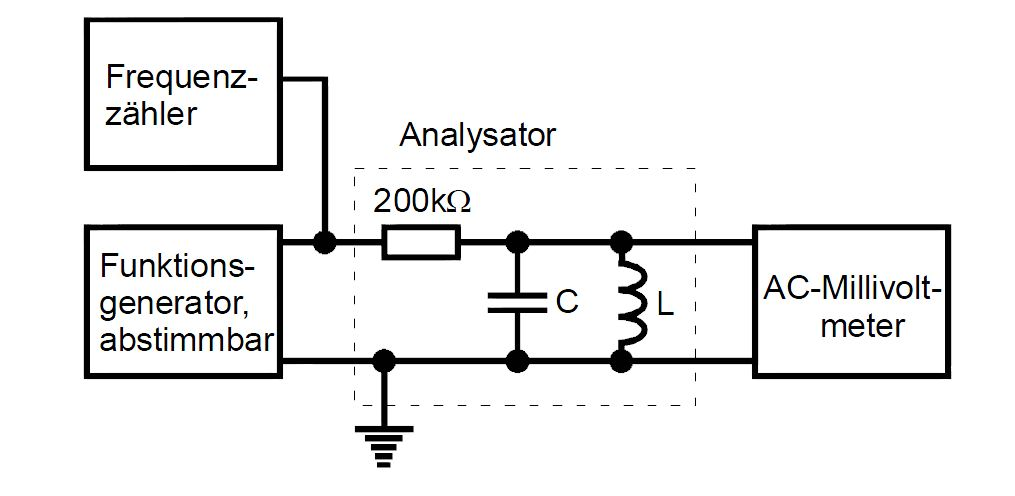
\includegraphics[scale=0.4]{picfouana.jpg}
		\caption{Schaltung zur Fourier-Analyse [1]}
		\label{picfouana}
		\end{center}	
	\end{figure}
Periodischen Funktionen $f$ mit der Periodendauer $T$ lassen sich durch Cosinus- und Sinusfunktionen
beschreiben (Gl. \ref{eqfou1}, \cite{anleitung}). Gleichheit in Gleichung (\ref{eqfou1}) gilt bei den meisten physikalischen Prozessen.
\begin{align}
f(t) &\sim \frac{a_0}{2} + \sum_{n=1}^{\infty} (a_n \text{ } cos(n \text{ } \frac{2 \pi}{T} t) + b_n \text{ } sin(n \frac{2 \pi}{T}) t) \label{eqfou1} \\
a_n &= \frac{2}{T} \int_0^T f(t) cos(n \frac{2 \pi}{T} t) \text{ dt} \text{ , } n=1,2, \ldots \label{eqfoua}\\
b_n &= \frac{2}{T} \int_0^T f(t) sin(n \frac{2 \pi}{T} t) \text{ dt} \text{ , } n=1,2, \ldots \label{eqfoub}
\end{align}
Die Fourier-Analyse beschreibt das Ermitteln der Vorfaktoren, beziehungsweise der Amplituden $a_n$ und $b_n$ für bekannte Funktionen.
Dabei kann man sich zunutze machen, dass bei geraden Funktionen $f$ alle $b_n=0$ werden und bei
ungeraden Funktionen alle $a_n$ verschwinden. Die Darstellung der Amplituden in Abhängigkeit zu von der zugehörigen Frequenz $n/T$
heißt Frequenzspektrum. Ein solches lässt sich beispielsweise mit einer Schaltung wie in Abbildung (\ref{picfouana})
bestimmen, welche auf der Proportionalität zwischen Resonanzspannung und Amplitude der Oberwellen beruht.
\subsection{Fourier-Synthese}
Im Gegensatz dazu wird bei der Fourier-Synthese eine Funktion aus bekannten Koeffizienten zusammengesetzt.
Durch schrittweises Hinzufügen der einzelnen Summanden wird die Funktion angenähert. Bei der
praktischen Umsetzung können Lissajous-Figuren, Kurven, die bei einer Schwingungsüberlagerung entstehen, helfen, 
die Phase der einzelnen Komponenten zu kalibrieren.
\subsection{Gibbsches Phänomen}
Das Gibbsche Phänomen tritt auf, wenn die Funktion $f(t)$ Unstetigkeiten aufweist. An den Stellen
der Unstetigkeit tritt immer ein endlicher Über-, beziehungsweise Unterschwung auf, da diese Stellen
nicht approximiert werden können.
\subsection{Fourier-Transformation}
Mit der Fourier-Transformation lässt sich das gesamte Frequenzspektrum, unabhängig einer
möglichen Periodizität der Funktion, bestimmen. Ähnlich zu Gleichung (\ref{eqfou1}) lässt sich auch die 
Fourier-Transformation beschreiben.
\begin{align}
f(t)&=\frac{1}{2 \pi} \int_{-\infty}^{\infty} g(\nu) e^{-i \nu t} \text{ d}\nu \\
g(\nu)&=\int_{-\infty}^{\infty} f(t) e^{i \nu t} \text{ dt} \label{eqfout2}
\end{align}
